\documentclass[varwidth=true, border=2pt]{standalone}

\usepackage{tikz}
\usetikzlibrary{decorations.fractals}
\usepackage{pgfplots}

\begin{document}
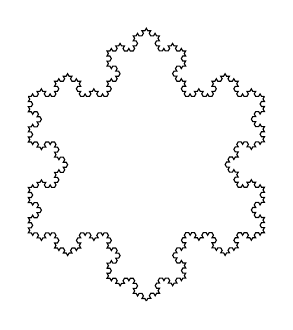
\begin{tikzpicture}[scale=3,decoration=Koch snowflake]
% \draw[fill=gray!10] { { { { (0,0) -- (3,0) -- (1.5,-3) -- (0,0)}}}};
% \draw[fill=gray!10] { { { decorate{ (0,0) -- (3,0) -- (1.5,-3) -- (0,0)}}}};
% \draw[fill=gray!10] { { decorate{ decorate{ (0,0) -- (3,0) -- (1.5,-3) -- (0,0)}}}};
% \draw[fill=gray!10] { decorate{ decorate{ decorate{ (0,0) -- (3,0) -- (1.5,-3) -- (0,0)}}}};
%\draw[fill=gray!10] decorate{ decorate{ decorate{ decorate{ (0,0) -- (3,0) -- (1.5,-3) -- (0,0)}}}};
%(0,0) -- (3,0) -- (1.5,-3) -- (0,0) does not form an equilateral triangle, so the Koch curves along (3,0) -- (1.5,-3) and (1.5,-3) -- (0,0) are longer than they should be

%using shifts and rotations makes an equilateral triangle easily without dealing explicitly with any irrational coordinates
\draw decorate{ decorate{ decorate{ decorate{ (0,0) -- (1,0) }}}};
\begin{scope}[shift={(1,0)}]
\begin{scope}[rotate=-120]
\draw decorate{ decorate{ decorate{ decorate{ (0,0) -- (1,0) }}}};
\end{scope}
\end{scope}
\begin{scope}[shift={(-1,0)}]
\begin{scope}[rotate around={120:(1,0)}]
\draw decorate{ decorate{ decorate{ decorate{ (0,0) -- (1,0) }}}};
\end{scope}
\end{scope}
\end{tikzpicture}
\end{document}
